% Created by tikzDevice version 0.6.2-92-0ad2792 on 2013-04-07 18:03:10
% !TEX encoding = UTF-8 Unicode
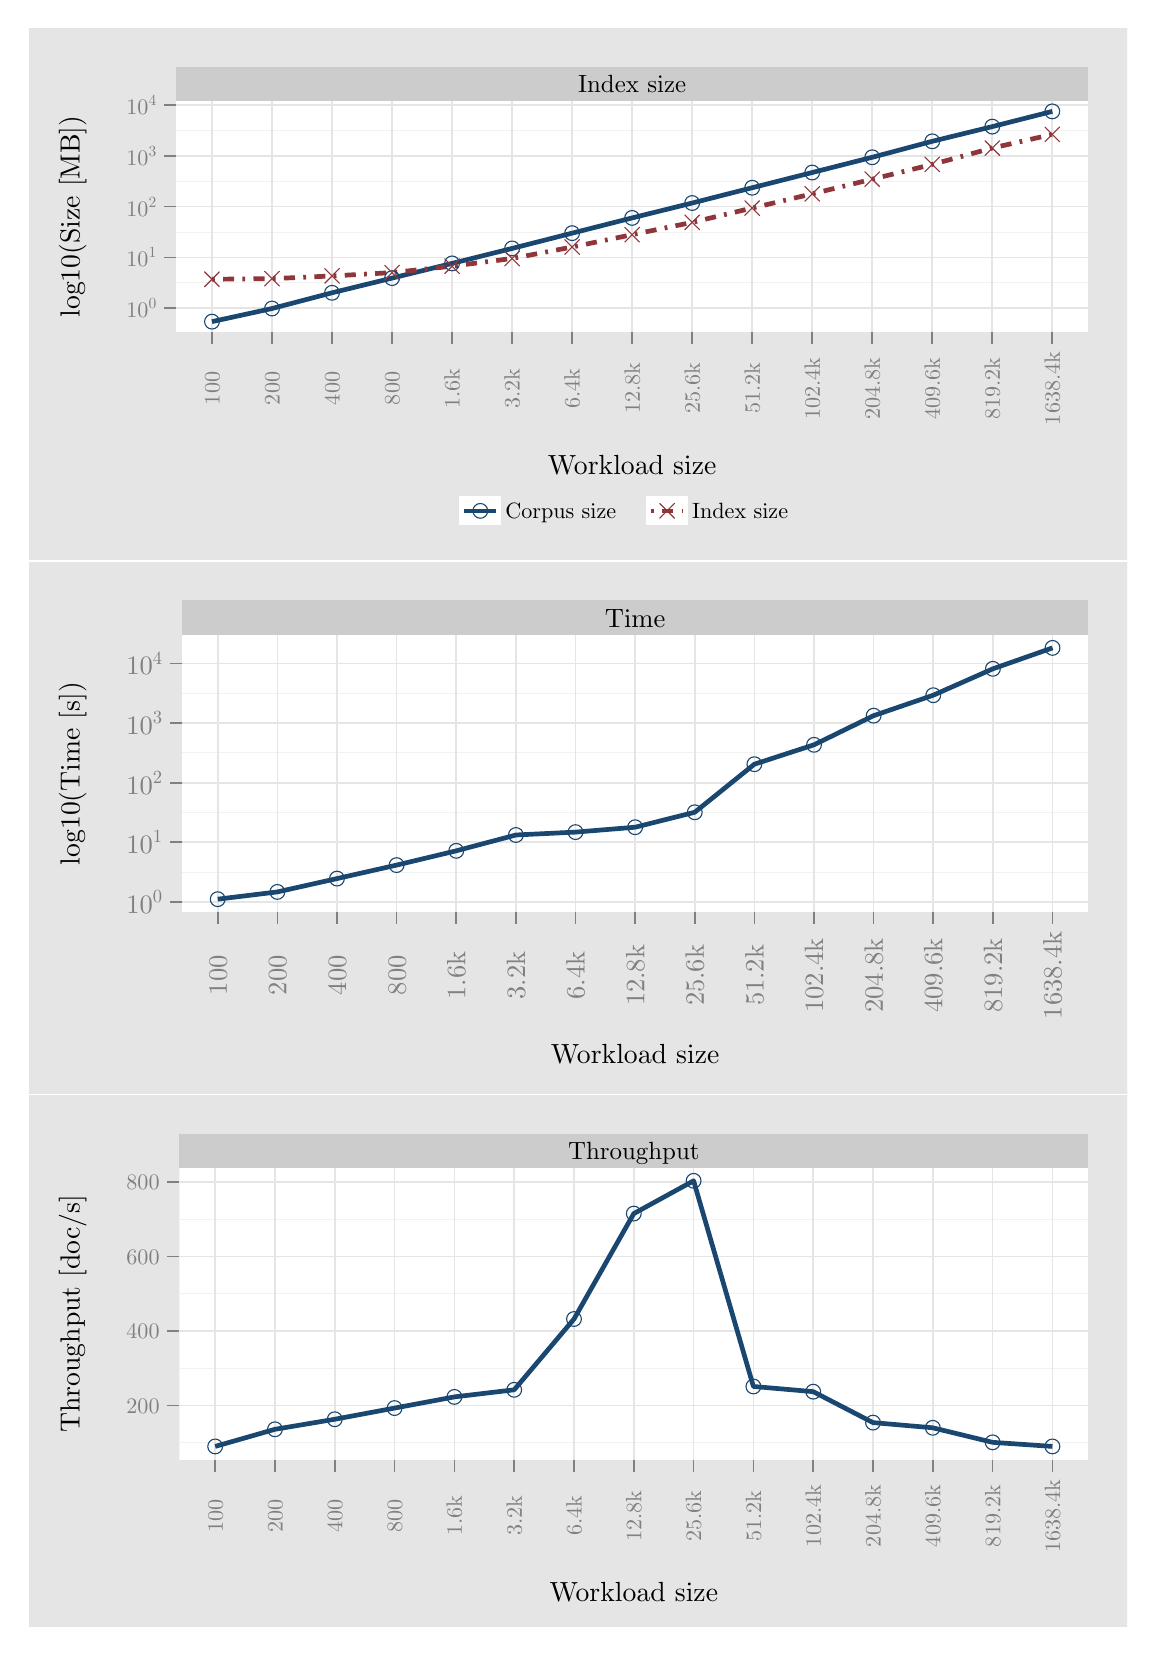
\begin{tikzpicture}[x=1pt,y=1pt]
\definecolor[named]{fillColor}{rgb}{1.00,1.00,1.00}
\path[use as bounding box,fill=fillColor,fill opacity=0.00] (0,0) rectangle (397.48,578.16);
\begin{scope}
\path[clip] (  0.00,385.44) rectangle (397.48,578.16);
\definecolor[named]{drawColor}{rgb}{1.00,1.00,1.00}
\definecolor[named]{fillColor}{rgb}{0.90,0.90,0.90}

\path[draw=drawColor,line width= 0.6pt,line join=round,line cap=round,fill=fillColor] (  0.00,385.44) rectangle (397.48,578.16);
\end{scope}
\begin{scope}
\path[clip] ( 53.58,468.13) rectangle (383.26,551.71);
\definecolor[named]{fillColor}{rgb}{1.00,1.00,1.00}

\path[fill=fillColor] ( 53.58,468.13) rectangle (383.26,551.71);
\definecolor[named]{drawColor}{rgb}{0.95,0.95,0.95}

\path[draw=drawColor,line width= 0.3pt,line join=round] ( 53.58,485.99) --
	(383.26,485.99);

\path[draw=drawColor,line width= 0.3pt,line join=round] ( 53.58,504.32) --
	(383.26,504.32);

\path[draw=drawColor,line width= 0.3pt,line join=round] ( 53.58,522.64) --
	(383.26,522.64);

\path[draw=drawColor,line width= 0.3pt,line join=round] ( 53.58,540.96) --
	(383.26,540.96);
\definecolor[named]{drawColor}{rgb}{0.90,0.90,0.90}

\path[draw=drawColor,line width= 0.6pt,line join=round] ( 53.58,476.83) --
	(383.26,476.83);

\path[draw=drawColor,line width= 0.6pt,line join=round] ( 53.58,495.15) --
	(383.26,495.15);

\path[draw=drawColor,line width= 0.6pt,line join=round] ( 53.58,513.48) --
	(383.26,513.48);

\path[draw=drawColor,line width= 0.6pt,line join=round] ( 53.58,531.80) --
	(383.26,531.80);

\path[draw=drawColor,line width= 0.6pt,line join=round] ( 53.58,550.12) --
	(383.26,550.12);

\path[draw=drawColor,line width= 0.6pt,line join=round] ( 66.60,468.13) --
	( 66.60,551.71);

\path[draw=drawColor,line width= 0.6pt,line join=round] ( 88.29,468.13) --
	( 88.29,551.71);

\path[draw=drawColor,line width= 0.6pt,line join=round] (109.97,468.13) --
	(109.97,551.71);

\path[draw=drawColor,line width= 0.6pt,line join=round] (131.66,468.13) --
	(131.66,551.71);

\path[draw=drawColor,line width= 0.6pt,line join=round] (153.35,468.13) --
	(153.35,551.71);

\path[draw=drawColor,line width= 0.6pt,line join=round] (175.04,468.13) --
	(175.04,551.71);

\path[draw=drawColor,line width= 0.6pt,line join=round] (196.73,468.13) --
	(196.73,551.71);

\path[draw=drawColor,line width= 0.6pt,line join=round] (218.42,468.13) --
	(218.42,551.71);

\path[draw=drawColor,line width= 0.6pt,line join=round] (240.11,468.13) --
	(240.11,551.71);

\path[draw=drawColor,line width= 0.6pt,line join=round] (261.80,468.13) --
	(261.80,551.71);

\path[draw=drawColor,line width= 0.6pt,line join=round] (283.49,468.13) --
	(283.49,551.71);

\path[draw=drawColor,line width= 0.6pt,line join=round] (305.18,468.13) --
	(305.18,551.71);

\path[draw=drawColor,line width= 0.6pt,line join=round] (326.87,468.13) --
	(326.87,551.71);

\path[draw=drawColor,line width= 0.6pt,line join=round] (348.56,468.13) --
	(348.56,551.71);

\path[draw=drawColor,line width= 0.6pt,line join=round] (370.25,468.13) --
	(370.25,551.71);
\definecolor[named]{drawColor}{rgb}{0.10,0.28,0.44}

\path[draw=drawColor,line width= 1.7pt,line join=round] ( 66.60,471.93) --
	( 88.29,476.67) --
	(109.97,482.35) --
	(131.66,487.66) --
	(153.35,492.97) --
	(175.04,498.38) --
	(196.73,503.90) --
	(218.42,509.41) --
	(240.11,514.79) --
	(261.80,520.31) --
	(283.49,525.81) --
	(305.18,531.32) --
	(326.87,537.09) --
	(348.56,542.40) --
	(370.25,547.91);
\definecolor[named]{drawColor}{rgb}{0.56,0.21,0.23}

\path[draw=drawColor,line width= 1.7pt,dash pattern=on 1pt off 3pt on 4pt off 3pt ,line join=round] ( 66.60,487.24) --
	( 88.29,487.46) --
	(109.97,488.44) --
	(131.66,489.64) --
	(153.35,491.97) --
	(175.04,494.75) --
	(196.73,498.89) --
	(218.42,503.35) --
	(240.11,507.80) --
	(261.80,512.98) --
	(283.49,518.11) --
	(305.18,523.40) --
	(326.87,528.73) --
	(348.56,534.66) --
	(370.25,539.59);
\definecolor[named]{drawColor}{rgb}{0.10,0.28,0.44}

\path[draw=drawColor,line width= 0.4pt,line join=round,line cap=round] ( 66.60,471.93) circle (  2.67);

\path[draw=drawColor,line width= 0.4pt,line join=round,line cap=round] ( 88.29,476.67) circle (  2.67);

\path[draw=drawColor,line width= 0.4pt,line join=round,line cap=round] (109.97,482.35) circle (  2.67);

\path[draw=drawColor,line width= 0.4pt,line join=round,line cap=round] (131.66,487.66) circle (  2.67);

\path[draw=drawColor,line width= 0.4pt,line join=round,line cap=round] (153.35,492.97) circle (  2.67);

\path[draw=drawColor,line width= 0.4pt,line join=round,line cap=round] (175.04,498.38) circle (  2.67);

\path[draw=drawColor,line width= 0.4pt,line join=round,line cap=round] (196.73,503.90) circle (  2.67);

\path[draw=drawColor,line width= 0.4pt,line join=round,line cap=round] (218.42,509.41) circle (  2.67);

\path[draw=drawColor,line width= 0.4pt,line join=round,line cap=round] (240.11,514.79) circle (  2.67);

\path[draw=drawColor,line width= 0.4pt,line join=round,line cap=round] (261.80,520.31) circle (  2.67);

\path[draw=drawColor,line width= 0.4pt,line join=round,line cap=round] (283.49,525.81) circle (  2.67);

\path[draw=drawColor,line width= 0.4pt,line join=round,line cap=round] (305.18,531.32) circle (  2.67);

\path[draw=drawColor,line width= 0.4pt,line join=round,line cap=round] (326.87,537.09) circle (  2.67);

\path[draw=drawColor,line width= 0.4pt,line join=round,line cap=round] (348.56,542.40) circle (  2.67);

\path[draw=drawColor,line width= 0.4pt,line join=round,line cap=round] (370.25,547.91) circle (  2.67);
\definecolor[named]{drawColor}{rgb}{0.56,0.21,0.23}

\path[draw=drawColor,line width= 0.4pt,line join=round,line cap=round,fill=fillColor] ( 63.93,484.58) -- ( 69.26,489.91);

\path[draw=drawColor,line width= 0.4pt,line join=round,line cap=round,fill=fillColor] ( 63.93,489.91) -- ( 69.26,484.58);

\path[draw=drawColor,line width= 0.4pt,line join=round,line cap=round,fill=fillColor] ( 85.62,484.79) -- ( 90.95,490.12);

\path[draw=drawColor,line width= 0.4pt,line join=round,line cap=round,fill=fillColor] ( 85.62,490.12) -- ( 90.95,484.79);

\path[draw=drawColor,line width= 0.4pt,line join=round,line cap=round,fill=fillColor] (107.31,485.77) -- (112.64,491.11);

\path[draw=drawColor,line width= 0.4pt,line join=round,line cap=round,fill=fillColor] (107.31,491.11) -- (112.64,485.77);

\path[draw=drawColor,line width= 0.4pt,line join=round,line cap=round,fill=fillColor] (129.00,486.97) -- (134.33,492.31);

\path[draw=drawColor,line width= 0.4pt,line join=round,line cap=round,fill=fillColor] (129.00,492.31) -- (134.33,486.97);

\path[draw=drawColor,line width= 0.4pt,line join=round,line cap=round,fill=fillColor] (150.69,489.30) -- (156.02,494.64);

\path[draw=drawColor,line width= 0.4pt,line join=round,line cap=round,fill=fillColor] (150.69,494.64) -- (156.02,489.30);

\path[draw=drawColor,line width= 0.4pt,line join=round,line cap=round,fill=fillColor] (172.37,492.08) -- (177.71,497.41);

\path[draw=drawColor,line width= 0.4pt,line join=round,line cap=round,fill=fillColor] (172.37,497.41) -- (177.71,492.08);

\path[draw=drawColor,line width= 0.4pt,line join=round,line cap=round,fill=fillColor] (194.06,496.23) -- (199.40,501.56);

\path[draw=drawColor,line width= 0.4pt,line join=round,line cap=round,fill=fillColor] (194.06,501.56) -- (199.40,496.23);

\path[draw=drawColor,line width= 0.4pt,line join=round,line cap=round,fill=fillColor] (215.75,500.68) -- (221.09,506.02);

\path[draw=drawColor,line width= 0.4pt,line join=round,line cap=round,fill=fillColor] (215.75,506.02) -- (221.09,500.68);

\path[draw=drawColor,line width= 0.4pt,line join=round,line cap=round,fill=fillColor] (237.44,505.13) -- (242.78,510.47);

\path[draw=drawColor,line width= 0.4pt,line join=round,line cap=round,fill=fillColor] (237.44,510.47) -- (242.78,505.13);

\path[draw=drawColor,line width= 0.4pt,line join=round,line cap=round,fill=fillColor] (259.13,510.32) -- (264.47,515.65);

\path[draw=drawColor,line width= 0.4pt,line join=round,line cap=round,fill=fillColor] (259.13,515.65) -- (264.47,510.32);

\path[draw=drawColor,line width= 0.4pt,line join=round,line cap=round,fill=fillColor] (280.82,515.44) -- (286.16,520.78);

\path[draw=drawColor,line width= 0.4pt,line join=round,line cap=round,fill=fillColor] (280.82,520.78) -- (286.16,515.44);

\path[draw=drawColor,line width= 0.4pt,line join=round,line cap=round,fill=fillColor] (302.51,520.73) -- (307.84,526.07);

\path[draw=drawColor,line width= 0.4pt,line join=round,line cap=round,fill=fillColor] (302.51,526.07) -- (307.84,520.73);

\path[draw=drawColor,line width= 0.4pt,line join=round,line cap=round,fill=fillColor] (324.20,526.06) -- (329.53,531.40);

\path[draw=drawColor,line width= 0.4pt,line join=round,line cap=round,fill=fillColor] (324.20,531.40) -- (329.53,526.06);

\path[draw=drawColor,line width= 0.4pt,line join=round,line cap=round,fill=fillColor] (345.89,532.00) -- (351.22,537.33);

\path[draw=drawColor,line width= 0.4pt,line join=round,line cap=round,fill=fillColor] (345.89,537.33) -- (351.22,532.00);

\path[draw=drawColor,line width= 0.4pt,line join=round,line cap=round,fill=fillColor] (367.58,536.92) -- (372.91,542.26);

\path[draw=drawColor,line width= 0.4pt,line join=round,line cap=round,fill=fillColor] (367.58,542.26) -- (372.91,536.92);
\end{scope}
\begin{scope}
\path[clip] (  0.00,  0.00) rectangle (397.48,578.16);
\definecolor[named]{fillColor}{rgb}{0.80,0.80,0.80}

\path[fill=fillColor] ( 53.58,551.71) rectangle (383.26,563.93);
\definecolor[named]{drawColor}{rgb}{0.00,0.00,0.00}

\node[text=drawColor,anchor=base,inner sep=0pt, outer sep=0pt, scale=  0.90] at (218.42,554.72) {Index size};
\end{scope}
\begin{scope}
\path[clip] (  0.00,  0.00) rectangle (397.48,578.16);
\definecolor[named]{drawColor}{rgb}{0.50,0.50,0.50}

\node[text=drawColor,anchor=base west,inner sep=0pt, outer sep=0pt, scale=  0.80] at ( 35.67,473.40) {10};

\node[text=drawColor,anchor=base west,inner sep=0pt, outer sep=0pt, scale=  0.56] at ( 43.67,476.67) {0};

\node[text=drawColor,anchor=base west,inner sep=0pt, outer sep=0pt, scale=  0.80] at ( 35.67,491.72) {10};

\node[text=drawColor,anchor=base west,inner sep=0pt, outer sep=0pt, scale=  0.56] at ( 43.67,494.99) {1};

\node[text=drawColor,anchor=base west,inner sep=0pt, outer sep=0pt, scale=  0.80] at ( 35.67,510.04) {10};

\node[text=drawColor,anchor=base west,inner sep=0pt, outer sep=0pt, scale=  0.56] at ( 43.67,513.32) {2};

\node[text=drawColor,anchor=base west,inner sep=0pt, outer sep=0pt, scale=  0.80] at ( 35.67,528.37) {10};

\node[text=drawColor,anchor=base west,inner sep=0pt, outer sep=0pt, scale=  0.56] at ( 43.67,531.64) {3};

\node[text=drawColor,anchor=base west,inner sep=0pt, outer sep=0pt, scale=  0.80] at ( 35.67,546.69) {10};

\node[text=drawColor,anchor=base west,inner sep=0pt, outer sep=0pt, scale=  0.56] at ( 43.67,549.96) {4};
\end{scope}
\begin{scope}
\path[clip] (  0.00,  0.00) rectangle (397.48,578.16);
\definecolor[named]{drawColor}{rgb}{0.50,0.50,0.50}

\path[draw=drawColor,line width= 0.6pt,line join=round] ( 49.31,476.83) --
	( 53.58,476.83);

\path[draw=drawColor,line width= 0.6pt,line join=round] ( 49.31,495.15) --
	( 53.58,495.15);

\path[draw=drawColor,line width= 0.6pt,line join=round] ( 49.31,513.48) --
	( 53.58,513.48);

\path[draw=drawColor,line width= 0.6pt,line join=round] ( 49.31,531.80) --
	( 53.58,531.80);

\path[draw=drawColor,line width= 0.6pt,line join=round] ( 49.31,550.12) --
	( 53.58,550.12);
\end{scope}
\begin{scope}
\path[clip] (  0.00,  0.00) rectangle (397.48,578.16);
\definecolor[named]{drawColor}{rgb}{0.50,0.50,0.50}

\path[draw=drawColor,line width= 0.6pt,line join=round] ( 66.60,463.86) --
	( 66.60,468.13);

\path[draw=drawColor,line width= 0.6pt,line join=round] ( 88.29,463.86) --
	( 88.29,468.13);

\path[draw=drawColor,line width= 0.6pt,line join=round] (109.97,463.86) --
	(109.97,468.13);

\path[draw=drawColor,line width= 0.6pt,line join=round] (131.66,463.86) --
	(131.66,468.13);

\path[draw=drawColor,line width= 0.6pt,line join=round] (153.35,463.86) --
	(153.35,468.13);

\path[draw=drawColor,line width= 0.6pt,line join=round] (175.04,463.86) --
	(175.04,468.13);

\path[draw=drawColor,line width= 0.6pt,line join=round] (196.73,463.86) --
	(196.73,468.13);

\path[draw=drawColor,line width= 0.6pt,line join=round] (218.42,463.86) --
	(218.42,468.13);

\path[draw=drawColor,line width= 0.6pt,line join=round] (240.11,463.86) --
	(240.11,468.13);

\path[draw=drawColor,line width= 0.6pt,line join=round] (261.80,463.86) --
	(261.80,468.13);

\path[draw=drawColor,line width= 0.6pt,line join=round] (283.49,463.86) --
	(283.49,468.13);

\path[draw=drawColor,line width= 0.6pt,line join=round] (305.18,463.86) --
	(305.18,468.13);

\path[draw=drawColor,line width= 0.6pt,line join=round] (326.87,463.86) --
	(326.87,468.13);

\path[draw=drawColor,line width= 0.6pt,line join=round] (348.56,463.86) --
	(348.56,468.13);

\path[draw=drawColor,line width= 0.6pt,line join=round] (370.25,463.86) --
	(370.25,468.13);
\end{scope}
\begin{scope}
\path[clip] (  0.00,  0.00) rectangle (397.48,578.16);
\definecolor[named]{drawColor}{rgb}{0.50,0.50,0.50}

\node[text=drawColor,rotate= 90.00,anchor=base,inner sep=0pt, outer sep=0pt, scale=  0.80] at ( 69.35,447.80) {100};

\node[text=drawColor,rotate= 90.00,anchor=base,inner sep=0pt, outer sep=0pt, scale=  0.80] at ( 91.04,447.80) {200};

\node[text=drawColor,rotate= 90.00,anchor=base,inner sep=0pt, outer sep=0pt, scale=  0.80] at (112.73,447.80) {400};

\node[text=drawColor,rotate= 90.00,anchor=base,inner sep=0pt, outer sep=0pt, scale=  0.80] at (134.42,447.80) {800};

\node[text=drawColor,rotate= 90.00,anchor=base,inner sep=0pt, outer sep=0pt, scale=  0.80] at (156.11,447.80) {1.6k};

\node[text=drawColor,rotate= 90.00,anchor=base,inner sep=0pt, outer sep=0pt, scale=  0.80] at (177.80,447.80) {3.2k};

\node[text=drawColor,rotate= 90.00,anchor=base,inner sep=0pt, outer sep=0pt, scale=  0.80] at (199.49,447.80) {6.4k};

\node[text=drawColor,rotate= 90.00,anchor=base,inner sep=0pt, outer sep=0pt, scale=  0.80] at (221.18,447.80) {12.8k};

\node[text=drawColor,rotate= 90.00,anchor=base,inner sep=0pt, outer sep=0pt, scale=  0.80] at (242.86,447.80) {25.6k};

\node[text=drawColor,rotate= 90.00,anchor=base,inner sep=0pt, outer sep=0pt, scale=  0.80] at (264.55,447.80) {51.2k};

\node[text=drawColor,rotate= 90.00,anchor=base,inner sep=0pt, outer sep=0pt, scale=  0.80] at (286.24,447.80) {102.4k};

\node[text=drawColor,rotate= 90.00,anchor=base,inner sep=0pt, outer sep=0pt, scale=  0.80] at (307.93,447.80) {204.8k};

\node[text=drawColor,rotate= 90.00,anchor=base,inner sep=0pt, outer sep=0pt, scale=  0.80] at (329.62,447.80) {409.6k};

\node[text=drawColor,rotate= 90.00,anchor=base,inner sep=0pt, outer sep=0pt, scale=  0.80] at (351.31,447.80) {819.2k};

\node[text=drawColor,rotate= 90.00,anchor=base,inner sep=0pt, outer sep=0pt, scale=  0.80] at (373.00,447.80) {1638.4k};
\end{scope}
\begin{scope}
\path[clip] (  0.00,  0.00) rectangle (397.48,578.16);
\definecolor[named]{drawColor}{rgb}{0.00,0.00,0.00}

\node[text=drawColor,anchor=base,inner sep=0pt, outer sep=0pt, scale=  1.00] at (218.42,416.85) {Workload size};
\end{scope}
\begin{scope}
\path[clip] (  0.00,  0.00) rectangle (397.48,578.16);
\definecolor[named]{drawColor}{rgb}{0.00,0.00,0.00}

\node[text=drawColor,rotate= 90.00,anchor=base,inner sep=0pt, outer sep=0pt, scale=  1.00] at ( 18.80,509.92) {log10(Size [MB])};
\end{scope}
\begin{scope}
\path[clip] (  0.00,  0.00) rectangle (397.48,578.16);
\definecolor[named]{fillColor}{rgb}{0.90,0.90,0.90}

\path[fill=fillColor] (148.45,394.31) rectangle (288.39,412.80);
\end{scope}
\begin{scope}
\path[clip] (  0.00,  0.00) rectangle (397.48,578.16);
\definecolor[named]{drawColor}{rgb}{1.00,1.00,1.00}
\definecolor[named]{fillColor}{rgb}{1.00,1.00,1.00}

\path[draw=drawColor,line width= 0.6pt,line join=round,line cap=round,fill=fillColor] (156.33,398.58) rectangle (170.78,408.53);
\end{scope}
\begin{scope}
\path[clip] (  0.00,  0.00) rectangle (397.48,578.16);
\definecolor[named]{drawColor}{rgb}{0.10,0.28,0.44}

\path[draw=drawColor,line width= 1.7pt,line join=round] (157.77,403.55) -- (169.34,403.55);
\end{scope}
\begin{scope}
\path[clip] (  0.00,  0.00) rectangle (397.48,578.16);
\definecolor[named]{drawColor}{rgb}{0.10,0.28,0.44}

\path[draw=drawColor,line width= 0.4pt,line join=round,line cap=round] (163.56,403.55) circle (  2.67);
\end{scope}
\begin{scope}
\path[clip] (  0.00,  0.00) rectangle (397.48,578.16);
\definecolor[named]{drawColor}{rgb}{1.00,1.00,1.00}
\definecolor[named]{fillColor}{rgb}{1.00,1.00,1.00}

\path[draw=drawColor,line width= 0.6pt,line join=round,line cap=round,fill=fillColor] (223.83,398.58) rectangle (238.28,408.53);
\end{scope}
\begin{scope}
\path[clip] (  0.00,  0.00) rectangle (397.48,578.16);
\definecolor[named]{drawColor}{rgb}{0.56,0.21,0.23}

\path[draw=drawColor,line width= 1.7pt,dash pattern=on 1pt off 3pt on 4pt off 3pt ,line join=round] (225.28,403.55) -- (236.84,403.55);
\end{scope}
\begin{scope}
\path[clip] (  0.00,  0.00) rectangle (397.48,578.16);
\definecolor[named]{drawColor}{rgb}{0.56,0.21,0.23}
\definecolor[named]{fillColor}{rgb}{1.00,1.00,1.00}

\path[draw=drawColor,line width= 0.4pt,line join=round,line cap=round,fill=fillColor] (228.39,400.89) -- (233.72,406.22);

\path[draw=drawColor,line width= 0.4pt,line join=round,line cap=round,fill=fillColor] (228.39,406.22) -- (233.72,400.89);
\end{scope}
\begin{scope}
\path[clip] (  0.00,  0.00) rectangle (397.48,578.16);
\definecolor[named]{drawColor}{rgb}{0.00,0.00,0.00}

\node[text=drawColor,anchor=base west,inner sep=0pt, outer sep=0pt, scale=  0.80] at (172.59,400.80) {Corpus size $\;\;\;$};
\end{scope}
\begin{scope}
\path[clip] (  0.00,  0.00) rectangle (397.48,578.16);
\definecolor[named]{drawColor}{rgb}{0.00,0.00,0.00}

\node[text=drawColor,anchor=base west,inner sep=0pt, outer sep=0pt, scale=  0.80] at (240.09,400.80) {Index size $\;\;\;$};
\end{scope}
\begin{scope}
\path[clip] (  0.00,192.72) rectangle (397.48,385.44);
\definecolor[named]{drawColor}{rgb}{1.00,1.00,1.00}
\definecolor[named]{fillColor}{rgb}{0.90,0.90,0.90}

\path[draw=drawColor,line width= 0.6pt,line join=round,line cap=round,fill=fillColor] (  0.00,192.72) rectangle (397.48,385.44);
\end{scope}
\begin{scope}
\path[clip] ( 55.74,258.70) rectangle (383.26,358.58);
\definecolor[named]{fillColor}{rgb}{1.00,1.00,1.00}

\path[fill=fillColor] ( 55.74,258.70) rectangle (383.26,358.58);
\definecolor[named]{drawColor}{rgb}{0.95,0.95,0.95}

\path[draw=drawColor,line width= 0.3pt,line join=round] ( 55.74,273.03) --
	(383.26,273.03);

\path[draw=drawColor,line width= 0.3pt,line join=round] ( 55.74,294.56) --
	(383.26,294.56);

\path[draw=drawColor,line width= 0.3pt,line join=round] ( 55.74,316.10) --
	(383.26,316.10);

\path[draw=drawColor,line width= 0.3pt,line join=round] ( 55.74,337.64) --
	(383.26,337.64);
\definecolor[named]{drawColor}{rgb}{0.90,0.90,0.90}

\path[draw=drawColor,line width= 0.6pt,line join=round] ( 55.74,262.26) --
	(383.26,262.26);

\path[draw=drawColor,line width= 0.6pt,line join=round] ( 55.74,283.80) --
	(383.26,283.80);

\path[draw=drawColor,line width= 0.6pt,line join=round] ( 55.74,305.33) --
	(383.26,305.33);

\path[draw=drawColor,line width= 0.6pt,line join=round] ( 55.74,326.87) --
	(383.26,326.87);

\path[draw=drawColor,line width= 0.6pt,line join=round] ( 55.74,348.41) --
	(383.26,348.41);

\path[draw=drawColor,line width= 0.6pt,line join=round] ( 68.67,258.70) --
	( 68.67,358.58);

\path[draw=drawColor,line width= 0.6pt,line join=round] ( 90.22,258.70) --
	( 90.22,358.58);

\path[draw=drawColor,line width= 0.6pt,line join=round] (111.76,258.70) --
	(111.76,358.58);

\path[draw=drawColor,line width= 0.6pt,line join=round] (133.31,258.70) --
	(133.31,358.58);

\path[draw=drawColor,line width= 0.6pt,line join=round] (154.86,258.70) --
	(154.86,358.58);

\path[draw=drawColor,line width= 0.6pt,line join=round] (176.41,258.70) --
	(176.41,358.58);

\path[draw=drawColor,line width= 0.6pt,line join=round] (197.95,258.70) --
	(197.95,358.58);

\path[draw=drawColor,line width= 0.6pt,line join=round] (219.50,258.70) --
	(219.50,358.58);

\path[draw=drawColor,line width= 0.6pt,line join=round] (241.05,258.70) --
	(241.05,358.58);

\path[draw=drawColor,line width= 0.6pt,line join=round] (262.59,258.70) --
	(262.59,358.58);

\path[draw=drawColor,line width= 0.6pt,line join=round] (284.14,258.70) --
	(284.14,358.58);

\path[draw=drawColor,line width= 0.6pt,line join=round] (305.69,258.70) --
	(305.69,358.58);

\path[draw=drawColor,line width= 0.6pt,line join=round] (327.24,258.70) --
	(327.24,358.58);

\path[draw=drawColor,line width= 0.6pt,line join=round] (348.78,258.70) --
	(348.78,358.58);

\path[draw=drawColor,line width= 0.6pt,line join=round] (370.33,258.70) --
	(370.33,358.58);
\definecolor[named]{drawColor}{rgb}{0.10,0.28,0.44}

\path[draw=drawColor,line width= 1.7pt,line join=round] ( 68.67,263.24) --
	( 90.22,265.86) --
	(111.76,270.68) --
	(133.31,275.55) --
	(154.86,280.71) --
	(176.41,286.43) --
	(197.95,287.47) --
	(219.50,289.24) --
	(241.05,294.64) --
	(262.59,312.01) --
	(284.14,319.02) --
	(305.69,329.55) --
	(327.24,336.94) --
	(348.78,346.48) --
	(370.33,354.04);

\path[draw=drawColor,line width= 0.4pt,line join=round,line cap=round] ( 68.67,263.24) circle (  2.67);

\path[draw=drawColor,line width= 0.4pt,line join=round,line cap=round] ( 90.22,265.86) circle (  2.67);

\path[draw=drawColor,line width= 0.4pt,line join=round,line cap=round] (111.76,270.68) circle (  2.67);

\path[draw=drawColor,line width= 0.4pt,line join=round,line cap=round] (133.31,275.55) circle (  2.67);

\path[draw=drawColor,line width= 0.4pt,line join=round,line cap=round] (154.86,280.71) circle (  2.67);

\path[draw=drawColor,line width= 0.4pt,line join=round,line cap=round] (176.41,286.43) circle (  2.67);

\path[draw=drawColor,line width= 0.4pt,line join=round,line cap=round] (197.95,287.47) circle (  2.67);

\path[draw=drawColor,line width= 0.4pt,line join=round,line cap=round] (219.50,289.24) circle (  2.67);

\path[draw=drawColor,line width= 0.4pt,line join=round,line cap=round] (241.05,294.64) circle (  2.67);

\path[draw=drawColor,line width= 0.4pt,line join=round,line cap=round] (262.59,312.01) circle (  2.67);

\path[draw=drawColor,line width= 0.4pt,line join=round,line cap=round] (284.14,319.02) circle (  2.67);

\path[draw=drawColor,line width= 0.4pt,line join=round,line cap=round] (305.69,329.55) circle (  2.67);

\path[draw=drawColor,line width= 0.4pt,line join=round,line cap=round] (327.24,336.94) circle (  2.67);

\path[draw=drawColor,line width= 0.4pt,line join=round,line cap=round] (348.78,346.48) circle (  2.67);

\path[draw=drawColor,line width= 0.4pt,line join=round,line cap=round] (370.33,354.04) circle (  2.67);
\end{scope}
\begin{scope}
\path[clip] (  0.00,  0.00) rectangle (397.48,578.16);
\definecolor[named]{fillColor}{rgb}{0.80,0.80,0.80}

\path[fill=fillColor] ( 55.74,358.58) rectangle (383.26,371.21);
\definecolor[named]{drawColor}{rgb}{0.00,0.00,0.00}

\node[text=drawColor,anchor=base,inner sep=0pt, outer sep=0pt, scale=  0.96] at (219.50,361.59) {Time};
\end{scope}
\begin{scope}
\path[clip] (  0.00,  0.00) rectangle (397.48,578.16);
\definecolor[named]{drawColor}{rgb}{0.50,0.50,0.50}

\node[text=drawColor,anchor=base west,inner sep=0pt, outer sep=0pt, scale=  0.96] at ( 35.67,258.14) {10};

\node[text=drawColor,anchor=base west,inner sep=0pt, outer sep=0pt, scale=  0.67] at ( 45.27,262.07) {0};

\node[text=drawColor,anchor=base west,inner sep=0pt, outer sep=0pt, scale=  0.96] at ( 35.67,279.68) {10};

\node[text=drawColor,anchor=base west,inner sep=0pt, outer sep=0pt, scale=  0.67] at ( 45.27,283.60) {1};

\node[text=drawColor,anchor=base west,inner sep=0pt, outer sep=0pt, scale=  0.96] at ( 35.67,301.21) {10};

\node[text=drawColor,anchor=base west,inner sep=0pt, outer sep=0pt, scale=  0.67] at ( 45.27,305.14) {2};

\node[text=drawColor,anchor=base west,inner sep=0pt, outer sep=0pt, scale=  0.96] at ( 35.67,322.75) {10};

\node[text=drawColor,anchor=base west,inner sep=0pt, outer sep=0pt, scale=  0.67] at ( 45.27,326.68) {3};

\node[text=drawColor,anchor=base west,inner sep=0pt, outer sep=0pt, scale=  0.96] at ( 35.67,344.29) {10};

\node[text=drawColor,anchor=base west,inner sep=0pt, outer sep=0pt, scale=  0.67] at ( 45.27,348.21) {4};
\end{scope}
\begin{scope}
\path[clip] (  0.00,  0.00) rectangle (397.48,578.16);
\definecolor[named]{drawColor}{rgb}{0.50,0.50,0.50}

\path[draw=drawColor,line width= 0.6pt,line join=round] ( 51.47,262.26) --
	( 55.74,262.26);

\path[draw=drawColor,line width= 0.6pt,line join=round] ( 51.47,283.80) --
	( 55.74,283.80);

\path[draw=drawColor,line width= 0.6pt,line join=round] ( 51.47,305.33) --
	( 55.74,305.33);

\path[draw=drawColor,line width= 0.6pt,line join=round] ( 51.47,326.87) --
	( 55.74,326.87);

\path[draw=drawColor,line width= 0.6pt,line join=round] ( 51.47,348.41) --
	( 55.74,348.41);
\end{scope}
\begin{scope}
\path[clip] (  0.00,  0.00) rectangle (397.48,578.16);
\definecolor[named]{drawColor}{rgb}{0.50,0.50,0.50}

\path[draw=drawColor,line width= 0.6pt,line join=round] ( 68.67,254.43) --
	( 68.67,258.70);

\path[draw=drawColor,line width= 0.6pt,line join=round] ( 90.22,254.43) --
	( 90.22,258.70);

\path[draw=drawColor,line width= 0.6pt,line join=round] (111.76,254.43) --
	(111.76,258.70);

\path[draw=drawColor,line width= 0.6pt,line join=round] (133.31,254.43) --
	(133.31,258.70);

\path[draw=drawColor,line width= 0.6pt,line join=round] (154.86,254.43) --
	(154.86,258.70);

\path[draw=drawColor,line width= 0.6pt,line join=round] (176.41,254.43) --
	(176.41,258.70);

\path[draw=drawColor,line width= 0.6pt,line join=round] (197.95,254.43) --
	(197.95,258.70);

\path[draw=drawColor,line width= 0.6pt,line join=round] (219.50,254.43) --
	(219.50,258.70);

\path[draw=drawColor,line width= 0.6pt,line join=round] (241.05,254.43) --
	(241.05,258.70);

\path[draw=drawColor,line width= 0.6pt,line join=round] (262.59,254.43) --
	(262.59,258.70);

\path[draw=drawColor,line width= 0.6pt,line join=round] (284.14,254.43) --
	(284.14,258.70);

\path[draw=drawColor,line width= 0.6pt,line join=round] (305.69,254.43) --
	(305.69,258.70);

\path[draw=drawColor,line width= 0.6pt,line join=round] (327.24,254.43) --
	(327.24,258.70);

\path[draw=drawColor,line width= 0.6pt,line join=round] (348.78,254.43) --
	(348.78,258.70);

\path[draw=drawColor,line width= 0.6pt,line join=round] (370.33,254.43) --
	(370.33,258.70);
\end{scope}
\begin{scope}
\path[clip] (  0.00,  0.00) rectangle (397.48,578.16);
\definecolor[named]{drawColor}{rgb}{0.50,0.50,0.50}

\node[text=drawColor,rotate= 90.00,anchor=base,inner sep=0pt, outer sep=0pt, scale=  0.96] at ( 71.98,235.72) {100};

\node[text=drawColor,rotate= 90.00,anchor=base,inner sep=0pt, outer sep=0pt, scale=  0.96] at ( 93.52,235.72) {200};

\node[text=drawColor,rotate= 90.00,anchor=base,inner sep=0pt, outer sep=0pt, scale=  0.96] at (115.07,235.72) {400};

\node[text=drawColor,rotate= 90.00,anchor=base,inner sep=0pt, outer sep=0pt, scale=  0.96] at (136.62,235.72) {800};

\node[text=drawColor,rotate= 90.00,anchor=base,inner sep=0pt, outer sep=0pt, scale=  0.96] at (158.16,235.72) {1.6k};

\node[text=drawColor,rotate= 90.00,anchor=base,inner sep=0pt, outer sep=0pt, scale=  0.96] at (179.71,235.72) {3.2k};

\node[text=drawColor,rotate= 90.00,anchor=base,inner sep=0pt, outer sep=0pt, scale=  0.96] at (201.26,235.72) {6.4k};

\node[text=drawColor,rotate= 90.00,anchor=base,inner sep=0pt, outer sep=0pt, scale=  0.96] at (222.81,235.72) {12.8k};

\node[text=drawColor,rotate= 90.00,anchor=base,inner sep=0pt, outer sep=0pt, scale=  0.96] at (244.35,235.72) {25.6k};

\node[text=drawColor,rotate= 90.00,anchor=base,inner sep=0pt, outer sep=0pt, scale=  0.96] at (265.90,235.72) {51.2k};

\node[text=drawColor,rotate= 90.00,anchor=base,inner sep=0pt, outer sep=0pt, scale=  0.96] at (287.45,235.72) {102.4k};

\node[text=drawColor,rotate= 90.00,anchor=base,inner sep=0pt, outer sep=0pt, scale=  0.96] at (308.99,235.72) {204.8k};

\node[text=drawColor,rotate= 90.00,anchor=base,inner sep=0pt, outer sep=0pt, scale=  0.96] at (330.54,235.72) {409.6k};

\node[text=drawColor,rotate= 90.00,anchor=base,inner sep=0pt, outer sep=0pt, scale=  0.96] at (352.09,235.72) {819.2k};

\node[text=drawColor,rotate= 90.00,anchor=base,inner sep=0pt, outer sep=0pt, scale=  0.96] at (373.64,235.72) {1638.4k};
\end{scope}
\begin{scope}
\path[clip] (  0.00,  0.00) rectangle (397.48,578.16);
\definecolor[named]{drawColor}{rgb}{0.00,0.00,0.00}

\node[text=drawColor,anchor=base,inner sep=0pt, outer sep=0pt, scale=  1.00] at (219.50,203.94) {Workload size};
\end{scope}
\begin{scope}
\path[clip] (  0.00,  0.00) rectangle (397.48,578.16);
\definecolor[named]{drawColor}{rgb}{0.00,0.00,0.00}

\node[text=drawColor,rotate= 90.00,anchor=base,inner sep=0pt, outer sep=0pt, scale=  1.00] at ( 18.80,308.64) {log10(Time [s])};
\end{scope}
\begin{scope}
\path[clip] (  0.00,  0.00) rectangle (397.48,192.72);
\definecolor[named]{drawColor}{rgb}{1.00,1.00,1.00}
\definecolor[named]{fillColor}{rgb}{0.90,0.90,0.90}

\path[draw=drawColor,line width= 0.6pt,line join=round,line cap=round,fill=fillColor] (  0.00,  0.00) rectangle (397.48,192.72);
\end{scope}
\begin{scope}
\path[clip] ( 54.78, 60.69) rectangle (383.26,166.27);
\definecolor[named]{fillColor}{rgb}{1.00,1.00,1.00}

\path[fill=fillColor] ( 54.78, 60.69) rectangle (383.26,166.27);
\definecolor[named]{drawColor}{rgb}{0.95,0.95,0.95}

\path[draw=drawColor,line width= 0.3pt,line join=round] ( 54.78, 66.83) --
	(383.26, 66.83);

\path[draw=drawColor,line width= 0.3pt,line join=round] ( 54.78, 93.76) --
	(383.26, 93.76);

\path[draw=drawColor,line width= 0.3pt,line join=round] ( 54.78,120.68) --
	(383.26,120.68);

\path[draw=drawColor,line width= 0.3pt,line join=round] ( 54.78,147.61) --
	(383.26,147.61);
\definecolor[named]{drawColor}{rgb}{0.90,0.90,0.90}

\path[draw=drawColor,line width= 0.6pt,line join=round] ( 54.78, 80.30) --
	(383.26, 80.30);

\path[draw=drawColor,line width= 0.6pt,line join=round] ( 54.78,107.22) --
	(383.26,107.22);

\path[draw=drawColor,line width= 0.6pt,line join=round] ( 54.78,134.14) --
	(383.26,134.14);

\path[draw=drawColor,line width= 0.6pt,line join=round] ( 54.78,161.07) --
	(383.26,161.07);

\path[draw=drawColor,line width= 0.6pt,line join=round] ( 67.75, 60.69) --
	( 67.75,166.27);

\path[draw=drawColor,line width= 0.6pt,line join=round] ( 89.36, 60.69) --
	( 89.36,166.27);

\path[draw=drawColor,line width= 0.6pt,line join=round] (110.97, 60.69) --
	(110.97,166.27);

\path[draw=drawColor,line width= 0.6pt,line join=round] (132.58, 60.69) --
	(132.58,166.27);

\path[draw=drawColor,line width= 0.6pt,line join=round] (154.19, 60.69) --
	(154.19,166.27);

\path[draw=drawColor,line width= 0.6pt,line join=round] (175.80, 60.69) --
	(175.80,166.27);

\path[draw=drawColor,line width= 0.6pt,line join=round] (197.41, 60.69) --
	(197.41,166.27);

\path[draw=drawColor,line width= 0.6pt,line join=round] (219.02, 60.69) --
	(219.02,166.27);

\path[draw=drawColor,line width= 0.6pt,line join=round] (240.63, 60.69) --
	(240.63,166.27);

\path[draw=drawColor,line width= 0.6pt,line join=round] (262.24, 60.69) --
	(262.24,166.27);

\path[draw=drawColor,line width= 0.6pt,line join=round] (283.85, 60.69) --
	(283.85,166.27);

\path[draw=drawColor,line width= 0.6pt,line join=round] (305.46, 60.69) --
	(305.46,166.27);

\path[draw=drawColor,line width= 0.6pt,line join=round] (327.07, 60.69) --
	(327.07,166.27);

\path[draw=drawColor,line width= 0.6pt,line join=round] (348.68, 60.69) --
	(348.68,166.27);

\path[draw=drawColor,line width= 0.6pt,line join=round] (370.29, 60.69) --
	(370.29,166.27);
\definecolor[named]{drawColor}{rgb}{0.10,0.28,0.44}

\path[draw=drawColor,line width= 1.7pt,line join=round] ( 67.75, 65.49) --
	( 89.36, 71.68) --
	(110.97, 75.31) --
	(132.58, 79.35) --
	(154.19, 83.39) --
	(175.80, 85.95) --
	(197.41,111.53) --
	(219.02,149.63) --
	(240.63,161.47) --
	(262.24, 87.16) --
	(283.85, 85.28) --
	(305.46, 74.10) --
	(327.07, 72.22) --
	(348.68, 66.97) --
	(370.29, 65.49);

\path[draw=drawColor,line width= 0.4pt,line join=round,line cap=round] ( 67.75, 65.49) circle (  2.67);

\path[draw=drawColor,line width= 0.4pt,line join=round,line cap=round] ( 89.36, 71.68) circle (  2.67);

\path[draw=drawColor,line width= 0.4pt,line join=round,line cap=round] (110.97, 75.31) circle (  2.67);

\path[draw=drawColor,line width= 0.4pt,line join=round,line cap=round] (132.58, 79.35) circle (  2.67);

\path[draw=drawColor,line width= 0.4pt,line join=round,line cap=round] (154.19, 83.39) circle (  2.67);

\path[draw=drawColor,line width= 0.4pt,line join=round,line cap=round] (175.80, 85.95) circle (  2.67);

\path[draw=drawColor,line width= 0.4pt,line join=round,line cap=round] (197.41,111.53) circle (  2.67);

\path[draw=drawColor,line width= 0.4pt,line join=round,line cap=round] (219.02,149.63) circle (  2.67);

\path[draw=drawColor,line width= 0.4pt,line join=round,line cap=round] (240.63,161.47) circle (  2.67);

\path[draw=drawColor,line width= 0.4pt,line join=round,line cap=round] (262.24, 87.16) circle (  2.67);

\path[draw=drawColor,line width= 0.4pt,line join=round,line cap=round] (283.85, 85.28) circle (  2.67);

\path[draw=drawColor,line width= 0.4pt,line join=round,line cap=round] (305.46, 74.10) circle (  2.67);

\path[draw=drawColor,line width= 0.4pt,line join=round,line cap=round] (327.07, 72.22) circle (  2.67);

\path[draw=drawColor,line width= 0.4pt,line join=round,line cap=round] (348.68, 66.97) circle (  2.67);

\path[draw=drawColor,line width= 0.4pt,line join=round,line cap=round] (370.29, 65.49) circle (  2.67);
\end{scope}
\begin{scope}
\path[clip] (  0.00,  0.00) rectangle (397.48,578.16);
\definecolor[named]{fillColor}{rgb}{0.80,0.80,0.80}

\path[fill=fillColor] ( 54.78,166.27) rectangle (383.26,178.49);
\definecolor[named]{drawColor}{rgb}{0.00,0.00,0.00}

\node[text=drawColor,anchor=base,inner sep=0pt, outer sep=0pt, scale=  0.90] at (219.02,169.28) {Throughput};
\end{scope}
\begin{scope}
\path[clip] (  0.00,  0.00) rectangle (397.48,578.16);
\definecolor[named]{drawColor}{rgb}{0.50,0.50,0.50}

\node[text=drawColor,anchor=base east,inner sep=0pt, outer sep=0pt, scale=  0.80] at ( 47.67, 77.54) {200};

\node[text=drawColor,anchor=base east,inner sep=0pt, outer sep=0pt, scale=  0.80] at ( 47.67,104.47) {400};

\node[text=drawColor,anchor=base east,inner sep=0pt, outer sep=0pt, scale=  0.80] at ( 47.67,131.39) {600};

\node[text=drawColor,anchor=base east,inner sep=0pt, outer sep=0pt, scale=  0.80] at ( 47.67,158.31) {800};
\end{scope}
\begin{scope}
\path[clip] (  0.00,  0.00) rectangle (397.48,578.16);
\definecolor[named]{drawColor}{rgb}{0.50,0.50,0.50}

\path[draw=drawColor,line width= 0.6pt,line join=round] ( 50.51, 80.30) --
	( 54.78, 80.30);

\path[draw=drawColor,line width= 0.6pt,line join=round] ( 50.51,107.22) --
	( 54.78,107.22);

\path[draw=drawColor,line width= 0.6pt,line join=round] ( 50.51,134.14) --
	( 54.78,134.14);

\path[draw=drawColor,line width= 0.6pt,line join=round] ( 50.51,161.07) --
	( 54.78,161.07);
\end{scope}
\begin{scope}
\path[clip] (  0.00,  0.00) rectangle (397.48,578.16);
\definecolor[named]{drawColor}{rgb}{0.50,0.50,0.50}

\path[draw=drawColor,line width= 0.6pt,line join=round] ( 67.75, 56.42) --
	( 67.75, 60.69);

\path[draw=drawColor,line width= 0.6pt,line join=round] ( 89.36, 56.42) --
	( 89.36, 60.69);

\path[draw=drawColor,line width= 0.6pt,line join=round] (110.97, 56.42) --
	(110.97, 60.69);

\path[draw=drawColor,line width= 0.6pt,line join=round] (132.58, 56.42) --
	(132.58, 60.69);

\path[draw=drawColor,line width= 0.6pt,line join=round] (154.19, 56.42) --
	(154.19, 60.69);

\path[draw=drawColor,line width= 0.6pt,line join=round] (175.80, 56.42) --
	(175.80, 60.69);

\path[draw=drawColor,line width= 0.6pt,line join=round] (197.41, 56.42) --
	(197.41, 60.69);

\path[draw=drawColor,line width= 0.6pt,line join=round] (219.02, 56.42) --
	(219.02, 60.69);

\path[draw=drawColor,line width= 0.6pt,line join=round] (240.63, 56.42) --
	(240.63, 60.69);

\path[draw=drawColor,line width= 0.6pt,line join=round] (262.24, 56.42) --
	(262.24, 60.69);

\path[draw=drawColor,line width= 0.6pt,line join=round] (283.85, 56.42) --
	(283.85, 60.69);

\path[draw=drawColor,line width= 0.6pt,line join=round] (305.46, 56.42) --
	(305.46, 60.69);

\path[draw=drawColor,line width= 0.6pt,line join=round] (327.07, 56.42) --
	(327.07, 60.69);

\path[draw=drawColor,line width= 0.6pt,line join=round] (348.68, 56.42) --
	(348.68, 60.69);

\path[draw=drawColor,line width= 0.6pt,line join=round] (370.29, 56.42) --
	(370.29, 60.69);
\end{scope}
\begin{scope}
\path[clip] (  0.00,  0.00) rectangle (397.48,578.16);
\definecolor[named]{drawColor}{rgb}{0.50,0.50,0.50}

\node[text=drawColor,rotate= 90.00,anchor=base,inner sep=0pt, outer sep=0pt, scale=  0.80] at ( 70.50, 40.36) {100};

\node[text=drawColor,rotate= 90.00,anchor=base,inner sep=0pt, outer sep=0pt, scale=  0.80] at ( 92.11, 40.36) {200};

\node[text=drawColor,rotate= 90.00,anchor=base,inner sep=0pt, outer sep=0pt, scale=  0.80] at (113.72, 40.36) {400};

\node[text=drawColor,rotate= 90.00,anchor=base,inner sep=0pt, outer sep=0pt, scale=  0.80] at (135.33, 40.36) {800};

\node[text=drawColor,rotate= 90.00,anchor=base,inner sep=0pt, outer sep=0pt, scale=  0.80] at (156.94, 40.36) {1.6k};

\node[text=drawColor,rotate= 90.00,anchor=base,inner sep=0pt, outer sep=0pt, scale=  0.80] at (178.55, 40.36) {3.2k};

\node[text=drawColor,rotate= 90.00,anchor=base,inner sep=0pt, outer sep=0pt, scale=  0.80] at (200.17, 40.36) {6.4k};

\node[text=drawColor,rotate= 90.00,anchor=base,inner sep=0pt, outer sep=0pt, scale=  0.80] at (221.78, 40.36) {12.8k};

\node[text=drawColor,rotate= 90.00,anchor=base,inner sep=0pt, outer sep=0pt, scale=  0.80] at (243.39, 40.36) {25.6k};

\node[text=drawColor,rotate= 90.00,anchor=base,inner sep=0pt, outer sep=0pt, scale=  0.80] at (265.00, 40.36) {51.2k};

\node[text=drawColor,rotate= 90.00,anchor=base,inner sep=0pt, outer sep=0pt, scale=  0.80] at (286.61, 40.36) {102.4k};

\node[text=drawColor,rotate= 90.00,anchor=base,inner sep=0pt, outer sep=0pt, scale=  0.80] at (308.22, 40.36) {204.8k};

\node[text=drawColor,rotate= 90.00,anchor=base,inner sep=0pt, outer sep=0pt, scale=  0.80] at (329.83, 40.36) {409.6k};

\node[text=drawColor,rotate= 90.00,anchor=base,inner sep=0pt, outer sep=0pt, scale=  0.80] at (351.44, 40.36) {819.2k};

\node[text=drawColor,rotate= 90.00,anchor=base,inner sep=0pt, outer sep=0pt, scale=  0.80] at (373.05, 40.36) {1638.4k};
\end{scope}
\begin{scope}
\path[clip] (  0.00,  0.00) rectangle (397.48,578.16);
\definecolor[named]{drawColor}{rgb}{0.00,0.00,0.00}

\node[text=drawColor,anchor=base,inner sep=0pt, outer sep=0pt, scale=  1.00] at (219.02,  9.41) {Workload size};
\end{scope}
\begin{scope}
\path[clip] (  0.00,  0.00) rectangle (397.48,578.16);
\definecolor[named]{drawColor}{rgb}{0.00,0.00,0.00}

\node[text=drawColor,rotate= 90.00,anchor=base,inner sep=0pt, outer sep=0pt, scale=  1.00] at ( 18.80,113.48) {Throughput [doc/s]};
\end{scope}
\end{tikzpicture}
